\chapter{Méthode CDLOD}
  \label{chap:cdlod}

  La méthode \emph{CDLOD}, pour "Continuous Distance-Dependent Level of Detail for Rendering Heightmaps" (Niveau de détail continu dépendant de la distance pour le rendu de carte de hauteur") par Filip Strugar~\cite{CDLOD}, 
  est un algorithme qui comme son nom l'indique, se base sur la distance entre la caméra et le terrain pour l'affichage du niveau de détail 
  (\textit{LOD}) basé sur une carte de hauteur (\emph{Heightmaps}).

  De nombreux algorithmes se servent de niveaux de détail pour générer leurs terrains. Mais, un de leurs problèmes majeurs est la gestion de la séparation entre deux niveaux de détail voisins.
  
 \begin{wrapfigure}[18]{r}{6cm}
 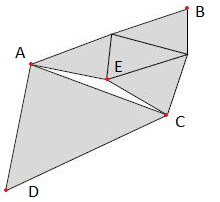
\includegraphics[width=6cm]{img/cracks.png}
   \caption[Discontinuité]{Discontinuité\protect\footnotemark}
   \label{fig:cracks}
 \end{wrapfigure}
 \footnotetext{Extrait de \url{https://people.eecs.berkeley.edu/~sequin/CS284/LECT09/L13.html}, dernier accès Mars 2018}
 
 \vspace{0.1cm}
 En effet la différence d'élévation entre chaque division peut provoquer une discontinuité dont résulte un trou. Sur la figure\ref{fig:cracks}, en se plaçant par exemple, dans le contexte d'une sphère lisse, lorsque le niveau de détails formés par le triangle ABC se divise en 4, pour améliorer le niveau de détails de ce dernier. Le point E, formé par le changement de niveau de détail, va venir se placer à la hauteur qui lui correspond (ici en s'élevant). Un nouveau triangle se crée alors entre les sommets communs des 2 niveaux de détails voisins et le nouveau point ajuster à sa hauteur(ici AEC). Comme ce triangle n'est pas le résultat d'une séparation/divisions d'un autre triangle, il ne possède pas de texture et crée ainsi un trou.\\
 
 
 La méthode utilisée en général pour pallier cette discontinuité est de rajouter des connexions entre les niveaux affectés. 
 Cette solution a de nombreux inconvénients, en rajoutant des connexions de cette manière, lors du rendu et, lors du parcours du terrain, ces connexions vont alors apparaître brusquement perturbant ainsi la continuité. À cela viennent s'ajouter la possibilité d'avoir des connexions multiples superposées et un coût supplémentaire en matière de calcul, mémoire et vitesse de rendu.
 
 L'algorithme CDLOD va notamment se différencier ici des autres algorithmes par ses "transitions fluides" entre les niveaux de détails par une méthode dite de "\textit{morphing}" dont nous reparlerons(section \ref{subsec:morphing} après avoir expliqué l'algorithme plus en détails.
 
 Pour pouvoir correctement expliquer l'algorithme il est tout d'abord nécessaire d'introduire les notions de  \textit{heightmap} ainsi que de \textit{quadtree} qui sont des éléments-clefs de l'algorithme.
 
  \section{Heightmap}
  \label{sec:heightmap}
  
  Une \emph{heightmap} pour "carte de hauteur" est une image permettant dans le cadre du rendu de terrain, de représenter le relief à l'aide de la nuance de gris. On peut ainsi interpréter la nuance comme une hauteur par rapport à la surface. Le noir représente la hauteur minimum et le blanc représente la hauteur maximum. Des algorithmes permettent d'obtenir une carte de hauteur ressemblant à des terrains naturels. Comme par exemple, l'algorithme de bruit de perlin, bruit de simplex , déplacement du point médian...
   
  
  
  
  \section{Quadtree}
  \label{sec:quadtree}
  
\begin{wrapfigure}[12]{r}{6cm}
 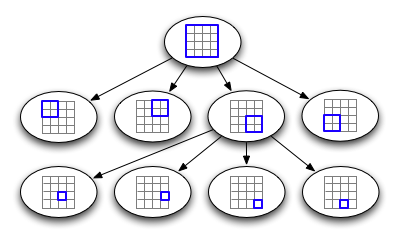
\includegraphics[width=6cm]{img/quadtree-arbre.png}
   \caption[Quadtree]{Quadtree\protect\footnotemark}
   \label{fig:quadtree-arbre}
 \end{wrapfigure}
 \footnotetext{Extrait de \url{http://codeforces.com/blog/entry/57498}, dernier accès Mars 2018}
  
 Un \emph{quadtree} est une structure de données s'apparentant à un arbre ou chaque n\oe{}ud de l'arbre possède quatre fils. Utiliser un \emph{quadtree} est un bon moyen de diviser un terrain 2D en plusieurs régions (représenter ici par la figure \ref{fig:quadtree-arbre}. Le terrain d'origine peut ainsi être divisé en quatre plus petites régions égales, puis chaque région obtenues en quatre sous-régions, et ainsi de suite, avec chaque n\oe{}ud comprenant des données correspondant à une sous-région. Pour à terme obtenir la région initial divisée en $4^n$ plus petite région de même taille avec n la hauteur de l'arbre.

  
\vspace{1.5cm}

\section{Continuous Distant-Dependent LOD ****}


  La méthode \textit{CDLOD}, est basé sur la méthode \textit{CLOD} "Chuncked LOD" développé par Thatcher Ulrich~\cite{CLOD} (dont nous proposons un résumé en annexe \ref{sec:chunked-lod}).
  

  Cette méthode organise une \emph{heightmap} dans un \emph{quadtree}, qui est utilisé pour sélectionner les niveaux de détails nécessaires au rendu. Lors de l'exécution le \emph{quadtree} est généré et composé des niveaux de détails, les \emph{LOD} nécessaires sont calculés et ainsi utilisés depuis le \emph{quadtree}. L'algorithme va assurer que le nombre de triangles affichés à l'écran reste constant, quelle que soit la distance entre la caméra et le terrain.
  
 \subsection{Sélection des n\oe{}uds dans le Quadtree ****}
 
    Pour pouvoir assurer que le nombre de triangles affichés à l'écran reste constant, il est nécessaire d'effectuer la sélection dans le \emph{quadtree} à chaque fois que la caméra bouge.\\
    \vspace{0.5cm}
    \begin{wrapfigure}[15]{r}{6cm}
 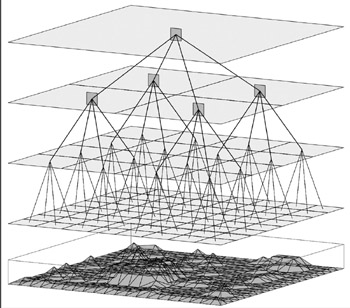
\includegraphics[width=6cm]{img/quadtree.png}
   \caption[Quadtree]{Quadtree\protect\footnotemark}
   \label{fig:quadtree-selection}
 \end{wrapfigure}
 \footnotetext{Extrait de \url{https://flylib.com/books/en/2.124.1.130/1/}, dernier accès Mars 2018}
    Le rendu du terrain est alors effectué en fonction de la distance entre le terrain et la caméra. Pour afficher un n\oe{}ud, le \emph{quadtree} est parcouru depuis la racine avec une tolérance maximale prédéfinie. Si le n\oe{}ud parcouru est valide il est affiché et s'il y a un trop grand écart alors on vérifie ses fils dans le \emph{quadtree}, et ainsi de suite. Les zones proches auront un niveau de détails élevé, alors que les zones plus lointaines seront moins détaillées. Le niveau de détails correspond alors à la profondeur dans le \emph{quadtree}, comme on peut l'observer sur la figure \ref{fig:quadtree-selection}

\newpage

\subsection{Intervention du Morphing ****}
\label{subsec:interventionMorphing}
    l'algorithme de CDLOD garde en continue un niveau de détail en utilisant sans arrêt des transitions. Contrairement à la méthode Chuncked-LOD de Ulrich.T ~\cite{CLOD} , Strugar.F dans sa méthode ~\cite{CDLOD}, n'utilise pas de "rideau" pour recouvrir le vide provoqué par la différence de niveau de détail, mais s'assure que le maillage du niveau supérieur soit complètement transformé en maillage de niveau inférieur avant que le changement ne se produise. Pour ce faire le \emph{morphing} expliqué dans la partie \ref{subsec:morphing} va être appliqué à chaque n\oe{}ud nécessitant l'augmentation ou la réduction de son niveau de détail. Afin de laisser une marge de mouvement au morphing pour arriver progressivement, la zone de transition couvre environ 15 à 30\% de chaque LOD. La figure \ref{fig:morph-area} montre les différents niveaux de transition du système de morphing, le niveau L1 étant le niveau le plus proche de la caméra et donc le niveau avec le plus de détail. On peut voir que les différents niveaux de transition ne sont pas linéaires en fonction de la distance.
\begin{figure}[!ht]
    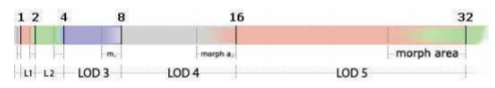
\includegraphics[width=12cm]{img/morph-area.png}
    \caption[morph-area]{Zone de transition \protect\footnotemark}
    \label{fig:morph-area}
\end{figure}
    \footnotetext{Extrait de \url{http://www.vertexasylum.com/downloads/cdlod/cdlod_latest.pdf}, dernier accès Mars 2018}

\subsection{Morphing ****}
\label{subsec:morphing}

  L'opération de \emph{morphing} est utilisée pour éviter l'apparition/disparition brusque des niveaux de détails. Chaque n\oe{}ud peut être transformé pour correspondre à un n\oe{}ud de niveau de détails plus élevé (en descendant plus profondément dans le \emph{quadtree} ou un niveau de détails moins élevé (en remontant dans le \emph{quadtree}. Le \emph{morphing} est réalisé de telle manière que chaque bloc de deux triangles sont  facilement transformés en un bloc correspondant de huit triangles. 
  
  Ce \emph{morphing} se traduira par des transitions en douceur sans discontinuité. Lors du rapprochement(ou éloignement) de la caméra par rapport au terrain, les sommets sont déplacés verticalement pour correspondre au niveau souhaité. Les transitions effectuées pour l'augmentation du niveau de détails sont représentées sur la figure \ref{fig:morph-transition}, expliquée ci-dessous. 
  
  On cherche à augmenter le niveau de détails du rectangle formé par les deux triangles \ref{subfig:morph-rectangle5}. Pour ce faire quatre nouveaux sommets vont être créés pour diviser le rectangle en quatre, puis vont se déplacer le long des arêtes afin que le point de jonction des rectangles suive la diagonale jusqu'au centre du rectangle (représenté par la ligne rouge \ref{subfig:morph-rectangle4} qui n'apparaît pas lors du rendu). Les rectangles vont ainsi grandir progressivement et sans discontinuité (observable sur les rectangles \ref{subfig:morph-rectangle4}, \ref{subfig:morph-rectangle3} et \ref{subfig:morph-rectangle2}) pour finalement diviser le rectangle d'origine en 4 nouveaux rectangles de même tailles, ayant donc augmenté son niveau de détail.
  
\begin{figure}[H]
    \centering
    \begin{subfigure}[b]{0.17\textwidth}
       \centering 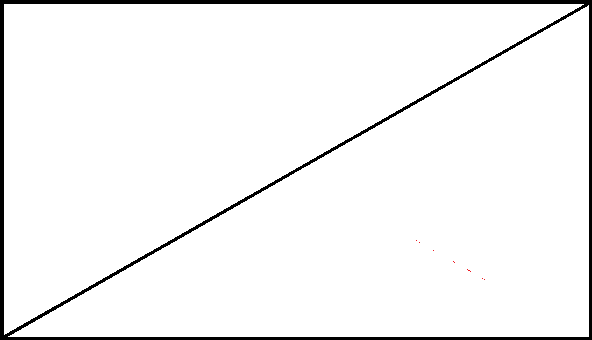
\includegraphics[width=\textwidth,height=1.3cm]{img/morph-rectangle5.png}
       \caption{}\label{subfig:morph-rectangle5}
    \end{subfigure}
    ~ 
    \begin{subfigure}[b]{0.17\textwidth}
       \centering 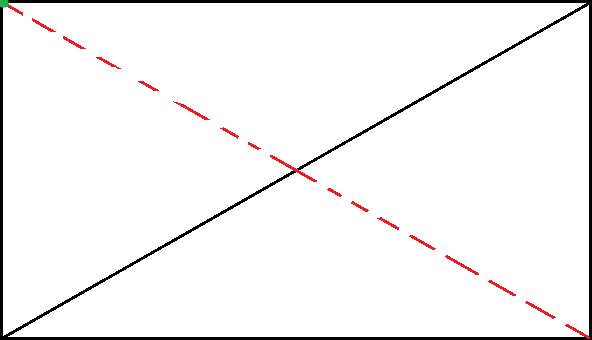
\includegraphics[width=\textwidth,height=1.3cm]{img/morph-rectangle4.png}
       \caption{}\label{subfig:morph-rectangle4}
    \end{subfigure}
    ~
    \begin{subfigure}[b]{0.17\textwidth}
       \centering 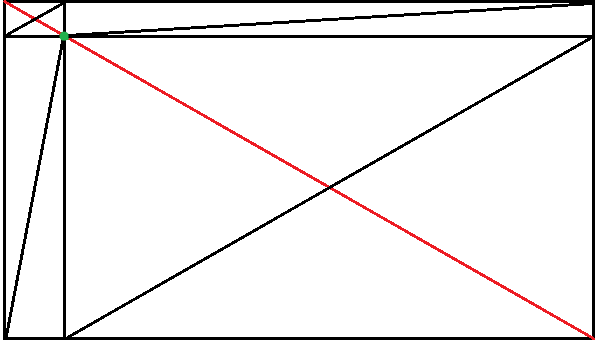
\includegraphics[width=\textwidth,height=1.3cm]{img/morph-rectangle3.png}
       \caption{}\label{subfig:morph-rectangle3}
    \end{subfigure}
    ~
    \begin{subfigure}[b]{0.16\textwidth}
       \centering 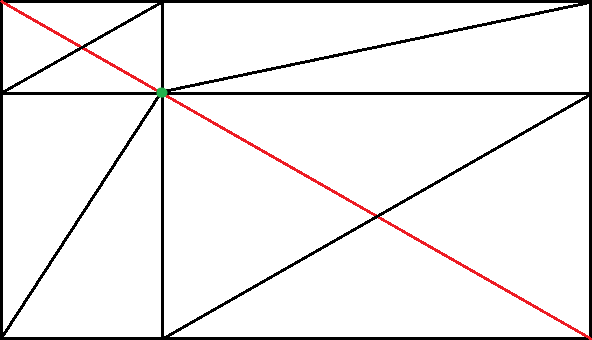
\includegraphics[width=\textwidth,height=1.3cm]{img/morph-rectangle2.png}
       \caption{}\label{subfig:morph-rectangle2}
    \end{subfigure}
     ~
    \begin{subfigure}[b]{0.16\textwidth}
       \centering 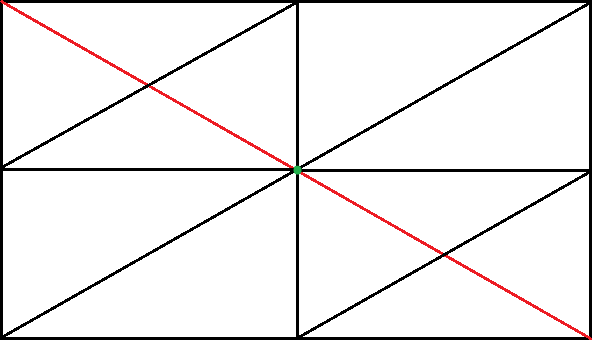
\includegraphics[width=\textwidth,height=1.3cm]{img/morph-rectangle1.png}
       \caption{}\label{subfig:morph-rectangle1}
    \end{subfigure}
    \caption{Morph sur des triangles}\label{fig:morph-transition}
\end{figure}



\subsection{Basic et Streaming Version}

    Il existe deux façons de stocker le Quadtree qui d'une version à l'autre réduit considérablement la mémoire utilisé. En effet la version BasicCDLOD assez simple à mettre en \oe{}uvre étend et stock entièrement tous les LOD, et, va venir parcourir la structure de données afin de sélectionner les niveaux nécessaires.
   
    Une autre version proposé, plus complexe à mettre en oeuvre mais qui économise grandement la mémoire, est la méthode StreamingCDLOD où seuls les parties nécessaires à la vue actuelle sont conservées. Les n\oe{}uds sont ensuite permutés si nécessaire. Par conséquent, les n\oe{}uds qui n'ont pas été utilisé pendant un certain temps peuvent être libérés.